\begin{figure}[t]
  \centering
   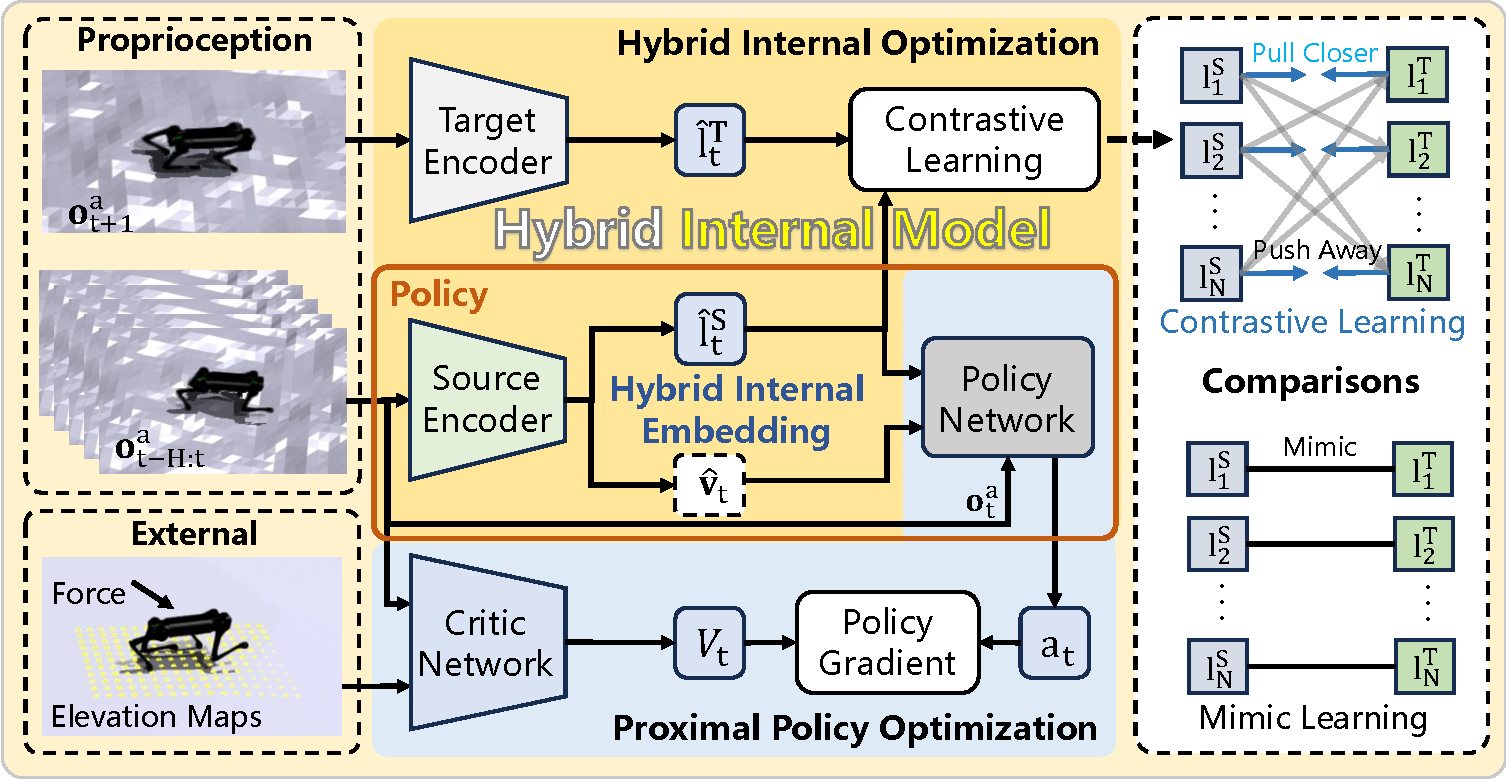
\includegraphics[width=1.0\linewidth]{overview.pdf}
   \caption{Overview of our framework. The policy network receives partial observations and the hybrid internal embedding, which is optimized to the robot's successor state with contrastive learning. The framework is alternatively optimized with HIO and PPO. }
   \label{fig:cl}
\end{figure}

\section{Methodology}
Our Hybrid Internal Model~(HIM) can efficiently train a policy that not only promotes sim2real compatibility but also significantly enhances robotic agility.
It is inspired by the classical Internal Model Control principles and implemented within a learning-based framework.
Next, we first present an overview and delve into details afterward.

\subsection{Framework Overview}
To control a legged robot, the algorithm needs to determine the movements of its actuators for a desired velocity given its proprioceptive information.
We follow the paradigm~\citep{rudin2022learning} that models the legged locomotion task as a sequential decision problem.
The entire framework is depicted in Fig.~\ref{fig:cl}.
The optimization process encompasses two phases: Hybrid Internal Optimization (HIO), which trains the hybrid internal model, and Proximal Policy Optimization (PPO), which optimizes the policy network.
In each iteration, we first update the parameters of HIM, then freeze them and optimize the actor and critic modules.

\paragraph{State Space.} 
The policy network takes partial observation $\mathbf{o}_{t}^{a}$ as input, which includes the desired velocity, the proprioceptive information from its joint encoder and IMU, and the last action $\mathbf{a}_{t-1}$.
The desired velocity $\mathbf{c}_t = [v_x^c, v_y^c, \omega_{\text{yaw}}^c]$ indicates the linear velocity in longitudinal and lateral directions, and the angular velocity in the horizontal direction, respectively. 
The joint encoder provides its joint position $\mathbf{\theta}_t$ and joint velocity $\dot{\mathbf{\theta}}_t$.
The IMU provides its base angular velocity $\mathbf{\omega}_t$ and gravity direction in robot frame $\mathbf{g}_t$.
Our value network is allowed to access privileged information at the training stage and thus can provide a more accurate estimation of state values.
Its input $\mathbf{o}_{t}^{c}$ contains two extra components to $\mathbf{o}_{t}^{a}$: current external force $\mathbf{f}_{t}$ and surrounding ground height $\mathbf{h}_{t}$.

\paragraph{Action Space.}
The movement of each actuator is formulated as the bias between the target joint position $\mathbf{\theta}_{\text{target}}$ and nominal joint position $\mathbf{\theta}_0$. 
To reduce the instability of the network output, we add a scale $k \leq 1$ to the policy output $\mathbf{a}_{t}$, thus the final target positions for joints are $\mathbf{\theta}_{\text{target}} = \mathbf{\theta}_0 + k \mathbf{a}_{t} .$
The dimension of the action space $\mathcal{A}$ equals the number of actuators. For example, quadrupedal robots such as Unitree A1 or ANYmal have 12 actuators, with 3 on each leg. 

\paragraph{Reward Functions.}
We follow the reward functions from~\cite{rudin2022learning} and~\cite{agarwal2023legged} with default weights. 
The details are listed in Appendix~\ref{app:rewards}.


\subsection{Hybrid Internal Model}
The classical Internal Model Control~(IMC)~\citep{rivera1986internal} suggests that we can perform robust control without directly modeling the disturbance. 
As shown in Fig~\ref{fig:imc}-(a), it uses an internal model to simulate the system response and further estimate the system disturbance, increasing the closed-loop stability. The more accurate the internal model is, the more robust control it can perform. 

\begin{wrapfigure}{r}{0.5\textwidth}
    % \vspace{-0.5cm}
    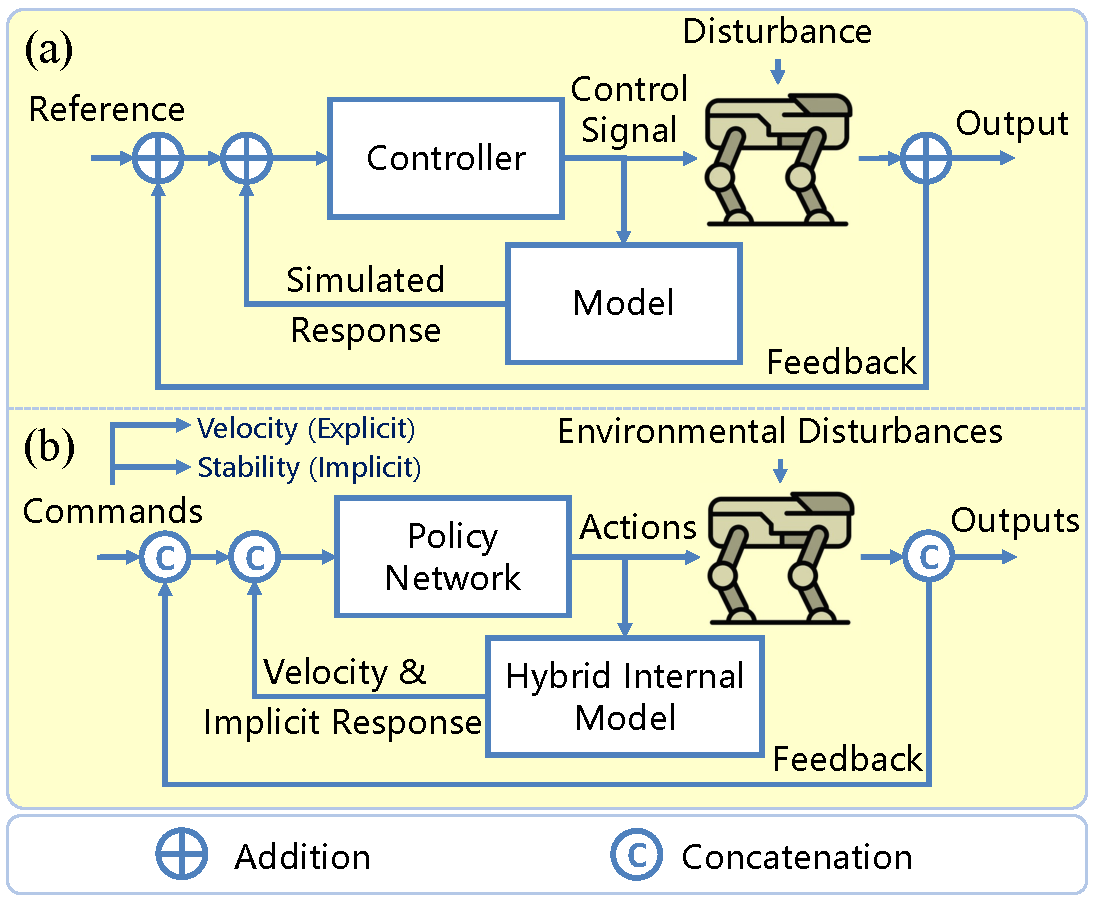
\includegraphics[width=0.5\textwidth]{imc.pdf}
    \vspace{-0.5cm}
    \caption{(a) IMC and (b) our implementations.}
    \vspace{-0.5cm}
    \label{fig:imc}
\end{wrapfigure}

In legged locomotion, the external environmental dynamics such as elevation maps, ground friction, and ground restitution are disturbances to the system. However, accurately estimating them is particularly challenging. Inspired by IMC, we propose using a model to estimate the robot's response as a viable alternative. As aforementioned, the robot is explicitly given a desired velocity for locomotion. Meanwhile, it is also implicitly commanded to maintain stability. To this end, we introduce a hybrid internal model that simultaneously estimates an explicit velocity and another implicit response. 
These estimations, along with robot observations, are collectively fed into the policy network, forming a fully closed-loop control system. The framework is shown in Fig~\ref{fig:imc}-(b).

In practice, HIM uses sequential history observations $\mathbf{o}_{t-H:t}^a$ to extract the hybrid internal embedding that consists of the robot's velocity $\hat{\mathbf{v}}_t$ and the implicit response $\mathbf{\hat{l}}_t$. H is set as 5 by default. 
The extractor is a 3-layer Multi-Layer Perceptron (MLP) with hidden dimensions of 512, 256, and 128, respectively.
The policy network takes the embedding and $\mathbf{o}_t^a$ as inputs and outputs actions. 


\subsection{Hybrid Internal Optimization}
The most critical thing for the internal embedding $(\hat{\mathbf{v}}_t, \mathbf{\hat{l}}_t)$ is how to optimize it to simulate the robot's response, which is naturally embedded within the robot's successor state $\mathbf{o}_{t+1}^{a}$.
In alignment with the principles of IMC, we can directly estimate $\mathbf{o}_{t+1}^a$ given $\mathbf{o}_{t-H:t}^a$.
However, this is challenging due to the high dimension of robot states and the disparity between simulation and reality.
Alternatively, given that we train the framework in a simulation environment, we can directly learn to regress the explicit velocity $\hat{\mathbf{v}}_t$ using its ground truth.
For the implicit response $\mathbf{\hat{l}}_t$, we propose modeling it into a latent space $\mathbf{Z} \subset \mathbf{R}^{16}$ and optimizing it to be close to the successor state with contrastive learning. 

In practice, in each iteration, we collect trajectories in each environment as a batch. 
If a pair of $\mathbf{o}_{t+1}^a$ and $\mathbf{o}_{t-H:t}^a$ belong to the same trajectory, they are positive pairs. Otherwise, they are negative pairs.
The pairs are optimized by swapping assignments tasks similar to SwAV~\citep{caron2020unsupervised}. 
% Instead of regression between a history of observations and the next observations in latent space, 
Given a sequence of proprioception observations sampled from the rollout trajectories, we can derive the subsequent observation $\mathbf{o}^a_{t+1}$ from a transition as a target vector and view the concatenated historical observations $\mathbf{o}^a_{t-H: t}$ as a source vector. 
We ensure that the augmentation is consistent across time steps. 
Source and target vectors are fed to the source encoder and target encoder respectively to obtain the latent feature $\mathbf{l}^{\text{source}}_t$ and $\mathbf{l}^{\text{target}}_t$ which are mapped onto a unit sphere in high-dimensional space with a $\mathcal{L}_2$-normalization.
To predict the cluster assignment probability $\mathbf{p}^{\text{source}}_t$ and $\mathbf{p}^{\text{target}}_t$ from $\mathbf{l}^{\text{source}}_t$ and $\mathbf{l}^{\text{target}}_t$, we first apply a $\mathcal{L}_2$-normalization on the prototype to obtain normalized matrix $\mathbf{E}=\{ \bar{\mathbf{e}}_1, ..., \bar{\mathbf{e}}_K \}$, and then take a softmax over the dot products of source vectors or target vectors with all the prototypes:
\begin{equation}
\begin{aligned}
    \mathbf{p}^{\text{source}}_t = \frac{\text{exp}(\frac{1}{\tau} {\mathbf{l}^{\text{source}}_t}^\top\mathbf{e}_k)}{\sum_{k'}\text{exp}(\frac{1}{\tau} {\mathbf{l}^{\text{source}}_t}^\top\mathbf{e}_{k'})},
\end{aligned}
\quad
\begin{aligned}
    \mathbf{p}^{\text{target}}_t = \frac{\text{exp}(\frac{1}{\tau} {\mathbf{l}^{\text{target}}_t}^\top\mathbf{e}_k)}{\sum_{k'}\text{exp}(\frac{1}{\tau} {\mathbf{l}^{\text{target}}_t}^\top\mathbf{e}_{k'})}.
\end{aligned}
\end{equation}
Here, $\mathbf{p}_t^{\text{source}}$ and $\mathbf{p}_t^{\text{target}}$ are the predicted probability that historical observations $\mathbf{o}^a_{t-H: t}$ maps to individual cluster with index $k$, while $\tau$ is a temperature parameter.


To obtain the targets $(\mathbf{q}^{\text{source}}_1, . . . , \mathbf{q}^{\text{source}}_K)$ and $(\mathbf{q}^{\text{target}}_1, . . . , \mathbf{q}^{\text{target}}_K)$ for the aforementioned predicted probabilities, while avoiding trivial solutions, the Sinkhorn-Knopp algorithm~\citep{cuturi2013sinkhorn} is applied to both encoders. Now that we have the cluster assignment predictions and targets, the representation learning objective is simply to maximize the prediction accuracy:

\begin{equation}
\mathcal{J}^{\text{SwAV}} = -\frac{1}{2H} \sum^{H}_{t=1} (\mathbf{q}^{\text{source}}_t \log \mathbf{p}^{\text{target}}_t + \mathbf{q}^{\text{target}}_t \log \mathbf{p}^{\text{source}}_t).
\end{equation}

\begin{figure}[t]
    \centering
    \vspace{-1cm}
    % \vspace*{-0.4cm}
    \subfigure[Ours]{
        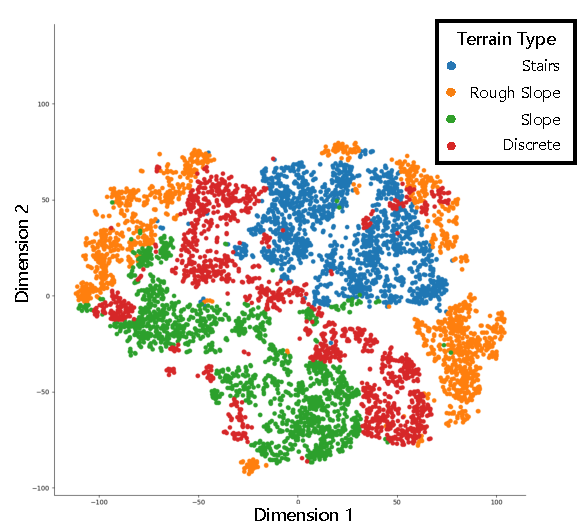
\includegraphics[width=0.36\textwidth]{tsne_him.pdf}
        \label{fig:cltsne}
    }
    \subfigure[Regression~\citep{nahrendra2023dreamwaq}]{
        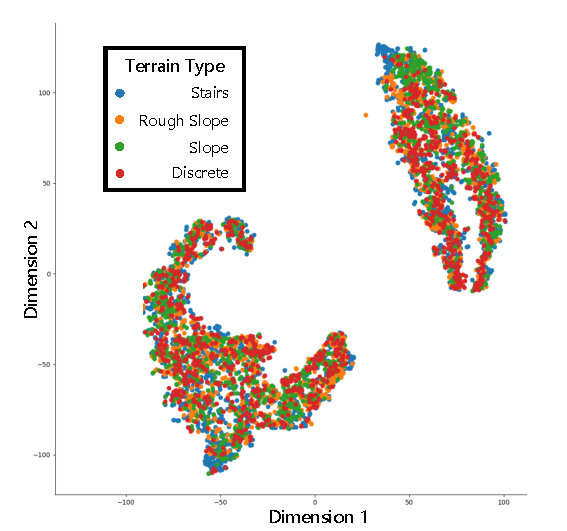
\includegraphics[width=0.36\textwidth]{tsne_reg.pdf}
        \label{fig:vae}
    }
    % \vspace*{-0.4cm}
    \caption{Latent space visualizations of (a) our hybrid internal model and (b)~\cite{nahrendra2023dreamwaq}.}
    \label{fig:main}
\end{figure}

\paragraph{Analysis.}
Our method can maximize the similarity of latent features between historical observations and the next observations, implicitly modeling external states without requirements for regression. This also improves the performance of locomotion policy by making use of the information in batch level, \emph{i.e.}, the different environment properties in different kinds of terrain. 
We conduct t-SNE~\cite{van2008visualizing} on the latent outputs of our methods and regression ~\citep{nahrendra2023dreamwaq}. The visualization shows that our hybrid internal model has a more separable encoding of environments, which means that our method carries more precious environmental information, resulting in a stronger ability to identify which kind of terrain the robot is on.




\subsection{Training Details}

\paragraph{Simulation Setup.}
We use Isaac Gym~\citep{rudin2022learning} with 4096 parallel environments and a rollout length of 100 time steps. The training process needs 1000 rollouts which takes 1 hour of wall clock time on NVIDIA RTX 4090. But its performance continues improving until 2000 rollouts.

\paragraph{Dynamics Randomization.}
To improve the robustness of the policy and facilitate the sim-to-real process, we randomize the mass of the robot body and links, the centre of mass (CoM) of the robot, the payload applied to the body of the robot, the ground friction and restitution coefficients, the motor strength, the joint-level PD gains, the system delay, the external force, and the initial joint positions in each episode. The randomization ranges for each parameter are detailed in Appendix~\ref{app:rand}.

\paragraph{Training Curriculum.}
\label{curriculum}
We use a similar terrain curriculum as \cite{rudin2022learning} and \cite{wu2023learning}. We create a height field map with $200$ terrains arranged in a $20 \times 10$ grid, and each row has the same type of terrain arranged in increasing difficulty, while each grid is $10 \times 10 \, \text{m}^2$. The detailed description of our training terrain is in Appendix~\ref{app:terrain}.  We put all the robots in different types of terrains with the lowest difficulty at the beginning, the terrain level will increase if the robot reaches 80\% of linear tracking reward, and will decrease if they can not travel half of the terrains in one episode.
We use a simple command curriculum to help the robots learn from easy to hard. On complex terrains such as stairs or discrete obstacles, we sample longitudinal and lateral linear velocity commands in $[-1.0,\, 1.0 ] \,\text{ m/s}$ and horizontal angular velocity in $[-2.0,\, 2.0 ]\,\text{ rad/s}$. On slopes and rough slopes, we increase the range of longitudinal linear velocity to $[-3.0,\, 3.0]\,\text{ m/s}$ and the range of horizontal angular velocity to $[-3.0,\, 3.0]\,\text{ rad/s}$. The commands are all sampled uniformly in the corresponding range and independently for each robot, we sample the commands every 25 time steps.
